\documentclass[11pt,a4paper,oneside]{report}

% Encodage et langue
\usepackage[utf8]{inputenc}
\usepackage[T1]{fontenc}
\usepackage[french]{babel}

% Polices modernes
\usepackage{lmodern}
\usepackage{mathpazo} % Utilisation de Palatino pour une apparence élégante
\linespread{1.05} % Augmenter légèrement l'interligne pour améliorer la lisibilité

% Mathématiques et graphiques
\usepackage{amsmath}
\usepackage{graphicx}
\usepackage{float}
\usepackage{tikz}

% Mise en page
\usepackage{geometry}
\geometry{left=2.0cm,right=2.0cm,top=2.0cm,bottom=2.0cm}

% En-têtes et pieds de page
\usepackage{fancyhdr}
\fancyhf{}
\renewcommand{\chaptermark}[1]{\markboth{#1}{}}
\rhead{\leftmark}
\cfoot{\thepage}
\renewcommand{\headrulewidth}{0.4pt}
\renewcommand{\footrulewidth}{0.4pt}

% Pour les pages spécifiques sans header et footer
\fancypagestyle{plain}{
    \fancyhf{}
    \renewcommand{\headrulewidth}{0pt}
    \renewcommand{\footrulewidth}{0pt}
}

% Titres
\title{Rapport d'Alternance}
\author{Paul Perigault}
\date{Mai 2024}

% Listes de code
\usepackage{listings}
\usepackage{xcolor}
\lstdefinestyle{mystyle}{
    backgroundcolor=\color{lightgray!20},
    commentstyle=\color{green},
    keywordstyle=\color{blue},
    numberstyle=\tiny\color{gray},
    stringstyle=\color{red},
    basicstyle=\ttfamily,
    inputencoding=utf8,
    extendedchars=false,
    breakatwhitespace=false,
    breaklines=true,
    captionpos=b,
    keepspaces=true,
    numbers=left,
    numbersep=5pt,
    showspaces=false,
    showstringspaces=false,
    showtabs=false,
    tabsize=2,
    literate= {á}{{\'a}}1
        {é}{{\'e}}1
        {í}{{\'i}}1
        {ó}{{\'o}}1
        {ú}{{\'u}}1
        {ê}{{\^e}}1
        {è}{{\`e}}1
}
\lstset{style=mystyle}

% Hyperliens
\usepackage[pdfborder={0 0 0}]{hyperref}

% Tableaux
\usepackage{array, tabularx, longtable, booktabs}

% Références
\usepackage{apalike}

% Table des matières et autres
\usepackage{minitoc}
\usepackage{enumitem}
\usepackage{epigraph}
\usepackage{lscape}
\usepackage{mdframed}
\mdfdefinestyle{summary}{
    innertopmargin=10pt,
    innerbottommargin=10pt,
    innerleftmargin=10pt,
    innerrightmargin=10pt,
    backgroundcolor=gray!10,
    linecolor=gray!50,
    linewidth=1pt,
    frametitleaboveskip=\dimexpr-\ht\strutbox\relax
}
\usepackage{emptypage}
\usepackage{multicol}
\usepackage{subcaption}

% Captions configuration
\usepackage{caption}
\captionsetup{font={sf, sl, small}, margin=3mm}
\captionsetup[lstlisting]{singlelinecheck=false}

% Personnalisation des sections et table des matières
\usepackage{titlesec}
\usepackage{tocloft}
\usepackage{sectsty}

% Couleurs personnalisées
\definecolor{chaptercolor}{RGB}{0, 102, 204}
\definecolor{subsectioncolor}{RGB}{0, 153, 51}
\definecolor{sectioncolor}{RGB}{204, 0, 102}

\chapterfont{\color{chaptercolor}}
\sectionfont{\color{sectioncolor}}
\subsectionfont{\color{subsectioncolor}}

% Table des matières personnalisée
\renewcommand{\cftsecfont}{\color{sectioncolor}}
\renewcommand{\cftsubsecfont}{\color{subsectioncolor}}
\renewcommand{\cftsecpagefont}{\color{sectioncolor}}
\renewcommand{\cftsubsecpagefont}{\color{subsectioncolor}}
\setlength{\cftbeforesecskip}{0pt}
\setlength{\cftbeforesubsecskip}{0pt}
\setlength{\cftaftertoctitleskip}{10pt} % Réduire l'espacement après le titre de la table des matières
\setlength{\cftbeforetoctitleskip}{10pt} % Réduire l'espacement avant le titre de la table des matières

% Optimisation
\newcommand{\anneeUniversitaire}{2023/2024}
\newcommand{\prenomNOM}{Perigault Paul}
\newcommand{\dateDebutAlternance}{04/09/2023}
\newcommand{\dateFinAlternance}{20/06/2024}
\newcommand{\nomEntreprise}{WeVii}
\newcommand{\sujetMission}{Alternance DevOps}
\newcommand{\tuteurAlternance}{Pascal Perigault}
\newcommand{\tuteurEcole}{Philipe Oliviero}

% Hauteur de l'en-tête
\setlength{\headheight}{15pt}

\begin{document}

    % Page de titre sans header/footer
    \thispagestyle{empty} % Utilisation de "empty" au lieu de "plain"
    \begin{titlepage}

    \newcommand{\HRule}{\rule{\linewidth}{0.5mm}} % épaisseur de lignes horizontales
    \setlength\fboxrule{2pt} % épaisseur de la boîte de mission

    \begin{center}
        % Logos et année universitaire

        \begin{minipage}{0.45\textwidth}
            \begin{flushleft}
                \href{https://iutparis-seine.u-paris.fr/}{
\includegraphics[width=5cm]{title/iutLogo}}
            \end{flushleft}
        \end{minipage}
        \hfill
        \begin{minipage}{0.45\textwidth}
            \begin{flushright}
                \href{https://www.wevii.net/}{
\includegraphics[width=3cm]{title/entrepriseLogo}}
            \end{flushright}
        \end{minipage}


        \vskip 1em
        \Large\textbf{ANNEE \anneeUniversitaire}

        % Titre principal
        \vskip 2em
        \Huge\textbf{RAPPORT D'ALTERNANCE}
        \vskip 0.5em
        \Large présenté par
        \vskip 0.5em
        \Huge\textbf{\prenomNOM}

        % Détails de la mission
        \vskip 2em
        \Large Mission effectuée du \dateDebutAlternance \ au \dateFinAlternance \ chez :
        \vskip 1em
        \Huge\textbf{\nomEntreprise}

        % Sujet de la mission
        \vskip 2em
        \Large Sujet de la mission :
        \vskip 0.5em
        \fbox{
            \begin{minipage}[c][3em]{0.9\textwidth}
                \centering
                \Large\textbf{\sujetMission}
            \end{minipage}
        }

        % Tuteurs
        \vskip 2em
        \begin{flushleft}
            \Large Tuteur entreprise : \textbf{\tuteurAlternance}
            \vskip 0.5em
            \Large Tuteur école : \textbf{\tuteurEcole}
        \end{flushleft}

        % Ligne horizontale
        \vskip 1em
        \HRule
    \end{center}

    \vfill % remplit le reste de la page avec des espaces

\end{titlepage}


    % Résumé sans header/footer
    \clearpage
    \thispagestyle{empty}
    \chapter*{\centering Résumé}
\addcontentsline{toc}{chapter}{Résumé}

\begin{mdframed}[style=summary]
    \noindent\textbf{Titre:} \textit{Alternance DevOps.}

    \vspace{0.2cm}
    \noindent\textbf{Mots clefs:} Alternance ; DevOps ; Cloud Computing ; Développement web ; Déploiement ;

    \vspace{0.3cm}
    \begin{multicols}{2}
        \noindent\textbf{Résumé:} \\
        Cette alternance au sein de la société WeVii, ESN Bordelaise et lilloise, m’a permis en tant qu’apprenti, d’être formé au métier du DevOps dans le domaine du cloud, en me donnant pour mission la réalisation de différents projets éducatifs sur ce thème.
        Mon premier projet se nommait Sandbox (Bac à sable) et le second Find Your Team (Trouve ton équipe).
        La réalisation de ces projets m’a permis d’acquérir les compétences nécessaires afin de participer pleinement à un projet de recherche et de développement porté par un professeur chercheur qui travaille sur un projet de R\&D (Recherche et Développement) pour la société WeVii Innovation, JEI (Jeune Entreprise Innovante), entreprise qui bénéficie du Crédit Impôt Recherche (CIR). Ces deux projets ont été menés à bien avec la méthodologie DevOps.
        Cette dernière est utilisée pour réaliser les projets grâce à différents outils tels que Typescript, Go, Docker, Kubernetes et Terraform.
        Ils ont été réalisés durant cette première année d’alternance.
        Ils m’ont permis une forte progression dans mon apprentissage car ils demandent une certaine rigueur et de nombreuses compétences.
        De plus, cela m’a aidé́ à me conforter dans mes choix et projets futurs.
    \end{multicols}
\end{mdframed}

\begin{mdframed}[style=summary]
    \noindent\textbf{Title:} \textit{Apprenticeship DevOps.}

    \vspace{0.2cm}
    \noindent\textbf{Keywords:} Work-Study ; DevOps ; Cloud Computing ; Web Development ; Deployment

    \vspace{0.3cm}
    \begin{multicols}{2}
        \noindent\textbf{Abstract:} \\
        As an apprentice at WeVii, an ESN based in Bordeaux and Lille, I was trained in DevOps in the cloud sector, and given the task of carrying out various educational projects on this theme.
        My first project was Sandbox, and my second was Find Your Team.
        The completion of these projects enabled me to acquire the skills needed to participate fully in a research and development project led by a research professor working on a R\&D (Research and Development) project for WeVii Innovation, a JEI (Jeune Entreprise Innovante), a company that benefits from the Crédit Impôt Recherche (CIR) tax credit. Both projects were carried out using DevOps methodology.
        This methodology is used to implement the projects using various tools such as Typescript, Go, Docker, Kubernetes and Terraform.
        These projects were carried out during my first year of work-study.
        They enabled me to make great progress in my apprenticeship, as they require a certain rigor and a number of skills.
        What's more, they helped mé to consolidate my choices and future projects.
    \end{multicols}
\end{mdframed}

\clearpage


    % Remerciements sans header/footer
    \clearpage
    \thispagestyle{empty}
    \chapter*{Remerciements}
\addcontentsline{toc}{chapter}{Remerciements}

Je remercie tout d’abord Nicolas Marie-Magdelaine pour son apport en compétences et son expertise de professeur chercheur qu’il n’a pas manqué de mettre à ma disposition.
Il a permis la réalisation des projets éducatifs en s’assurant de mon épanouissement professionnel tout au long de cette année avec un suivi hebdomadaire de qualité.

\bigskip

Je remercie aussi Cédric Maitre pour l’aide qu’il m’a apporté dans le suivi administratif, élément nouveau pour moi dans le cadre d’une expérience professionnelle.

\bigskip

Et également Denis Dormegnie, pour son accompagnement régulier et pour son expertise qu’il m’a partagé en tant que Chef de Projet et architecte technique.
\bigskip

Je tiens à remercier gracieusement l’ensemble du personnel de WeVii pour leur bienveillance.

\bigskip

Ainsi que l’ensemble du personnel enseignant de l’IUT Paris Rives de Seine.

\bigskip

Et particulièrement Philippe Oliviéro, mon tuteur enseignant, qui a su être présent pour moi au cours de cette année.

\bigskip

Pour finir, je remercie Pascal Perigault pour l’opportunité qu’il m’a proposé ainsi que pour le suivi quotidien dont il a fait part à mon égard.

\vfill % remplit le reste de la page avec des espaces

\clearpage


    % Table des matières sans header/footer
    \clearpage
    \thispagestyle{empty}
    \tableofcontents
    \clearpage

    % Sections principales avec numéro de page
    \pagestyle{fancy} % Appliquer l'en-tête personnalisé à partir de ce point
    \chapter*{Introduction}
\addcontentsline{toc}{chapter}{Introduction}

A la fin de ma première année en BUT informatique, j’ai eu la possibilité de poursuivre mon cursus en apprentissage.
La recherche d’une entreprise n’a pas été évidente mais au bout de plusieurs mois de recherche j’ai su saisir une très bonne opportunité qui correspondait à mes critères.
Cependant, je n’ai pas pris ma décision directement car l’entreprise se trouvant à Bordeaux il était clair qu’une grande partie de mon apprentissage se ferait en distanciel.
Après mûre réflexion et suite à de nombreuses discussions avec l’entreprise, j’ai su que le suivi allait être quotidien et que le projet avait beaucoup à m’apporter, j’ai donc accepté.

\bigskip

En effet, durant cette première année d’apprentissage, j’ai intégré l’Entreprise de Service Numérique (ESN) \textbf{WeVii} qui est située à Bordeaux.
Elle a pour modèle économique la prestation de service dans le numérique.
WeVii Bordeaux possède une filiale se nommant WeVii innovation.
Ainsi, j’ai intégré WeVii Bordeaux afin d’être formé pour sa filiale.

\bigskip

Pour ma part, j’interviens dans un des projets nommé, « TDC » (Tree Digital Cloud) qui est un projet de transformation digitale.
Mais pour cela j’ai dû être formé aux technologies du cloud tout en ayant une approche DevOps.

\bigskip

En somme, j'ai été formé aux technologies d’un projet afin d’y être intégré pleinement.
Globalement, les missions qui me sont confiées sont la réalisation de projets techniques, dans l’optique de me faire découvrir et progresser sur différentes technologies.

\bigskip

Depuis quelques années, j’ai pour projet de me diriger vers l’architecture cloud, pour devenir architecte cloud.
C’est un métier qui demande beaucoup de compétences car ses missions sont diverses.
Il doit savoir automatiser la gestion des infrastructures, développer des fonctionnalités pour ces dernières, mais aussi avoir des qualités de management afin de gérer des équipes.
J’aime l’idée de faire un métier pertinent, complet qui regroupe différents domaines, cela permet de ne pas se lasser.
J’ai accepté cette alternance car j’ai su que j’allais développer, ce qui me donne l’opportunité de savoir si j’apprécie réellement le développement et si le métier d’architecte cloud est vraiment ce qui me correspond.

\bigskip

Dans la suite de mon rapport, je vais vous présenter l’entreprise ainsi que les deux projets réalisés au cours de mon alternance.
En conclusion, nous ferons un point sur l’ensemble de cette année ainsi que sur les années futures.

\clearpage

    \pagestyle{fancy} % Appliquer l'en-tête personnalisé à partir de ce point
    \chapter{Environnement professionnel}

\section{L'entreprise}

\textbf{WeVii} est une Entreprise de Service du Numérique (ESN) créée en 2010 sous le nom d’AFIB Décision.
Son activité tournait autour de l’informatique décisionnelle.
En 2014, l’entreprise amorce un premier virage et se renomme \textbf{AFIB Services},
élargissant son activité à tous les services digitaux, et pas seulement au décisionnel. En 2019, face à des difficultés financières, l’entreprise est reprise par \textbf{Pascal Perigault} et \textbf{Romain Lavielle}, et devient \textbf{WeVii}.

\subsection{Évolution}

D’une situation critique avec quatre collaborateurs, l’entreprise s’est transformée pour atteindre aujourd’hui soixante-quinze collaborateurs répartis sur deux sites, Bordeaux et Lille, réalisant un chiffre d’affaires de sept millions d’euros.

\bigskip

\textbf{WeVii} est actuellement un groupe composé de huit entreprises :
\begin{itemize}
    \item Trois holdings : \textbf{Carat Conseil}, \textbf{Faerie Consulting}, et \textbf{WeVii Holding}.
    \item Les sociétés filles : \textbf{WeVii Bordeaux}, \textbf{WeVii Innovation}, \textbf{WeVii Paris}, \textbf{WeVii Lille}, et \textbf{WeVii Tech}.
\end{itemize}

\section{Les grandes dates}
\begin{figure}[H]
    \centering
    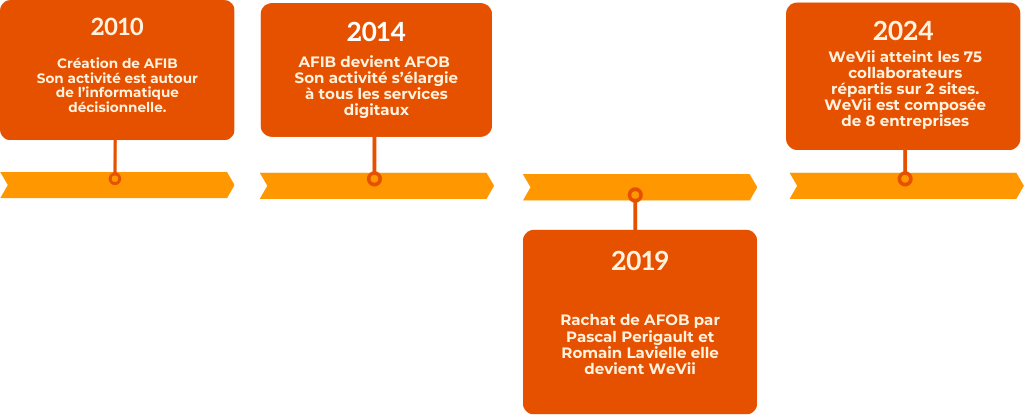
\includegraphics[width=\textwidth]{image/lesGrandesDates}
    \caption[Les grandes dates]{Les grandes dates de l'entreprise}
    \label{fig:grandes_dates}
\end{figure}

\section{Ma place dans l'entreprise}

Dans le cadre de cette transformation, \textbf{WeVii} lance des projets, dont un projet nommé \textbf{« TDC » (Tree Digital Cloud)}, porté par une nouvelle entreprise, \textbf{WeVii Innovation}, une JEI (Jeune Entreprise Innovante).
C’est pour ce projet, en tant que salarié de \textbf{WeVii Bordeaux}, que j’interviens dans le cadre de mon apprentissage.

\section{Organigramme de l'entreprise}
\begin{figure}[H]
    \centering
    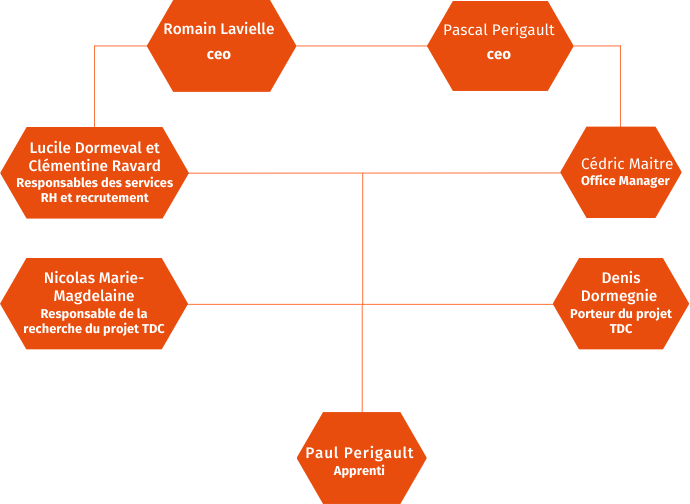
\includegraphics[width=\textwidth]{image/organigrammeEntreprise}
    \caption[Organigramme de l'entreprise]{Organigramme de l'entreprise}
    \label{fig:organigramme_entreprise}
\end{figure}

\section{Organisation de l'entreprise}

L'organisation du groupe est la suivante :
\begin{itemize}
    \item \textbf{Pascal Perigault} et \textbf{Romain Lavielle} sont les CEO.
    \item \textbf{Grégory Lacombe}, associé, dirige \textbf{WeVii Tech}, filiale de WeVii, nouvellement créée et spécialisée dans les métiers du cloud, de la sécurité et des opérations.
    \item \textbf{Lucile Dormeval} et \textbf{Clémentine Ravard} sont responsables des services RH et recrutement.
    \item \textbf{Cédric Maitre} est l'Office Manager (il dirige tout le back office).
    \item Les fonctions financières et paies sont sous-traitées par un cabinet spécialisé.
    \item \textbf{Nicolas Marie-Magdelaine}, Docteur en informatique, est responsable de la recherche du projet TDC. Il pilote mon activité technique.
    \item \textbf{Denis Dormegnie} est le porteur du projet TDC. Il pilote également mes projets.
\end{itemize}

\section{La vie en entreprise}

Durant la formation, mon outil de travail était un ordinateur portable MacBook Air fourni par l’entreprise.
J’ai été en grande partie en télétravail, bien que parfois je descendais à Bordeaux pour voir mes collègues et participer à la vie quotidienne et professionnelle de l’entreprise, afin de mieux m'intégrer.

\bigskip

Pour communiquer, nous utilisons \textbf{Teams}, un logiciel conçu par Microsoft permettant d’envoyer des messages, de faire des réunions à distance et de faciliter la communication inter-entreprise.
Malgré la distance, j’ai eu la chance de participer à la vie de l’entreprise, notamment en étant présent en visioconférence aux \textbf{WeTalkTech}, un podcast en direct où chaque intervenant présente une technologie ou un projet.

\bigskip

Les tâches m’étaient fournies par le chercheur, mais j’avais la possibilité d’ajouter une part de créativité.
J’utilisais la méthodologie \textbf{DevOps} pour construire et déployer mes projets tout en ayant une approche minimaliste apportée par le chercheur. Elles étaient sous forme de fonctionnalités et sous contraintes de temps, ce qui signifie que pour chaque élément à ajouter à l’application, nous estimons un temps pour le réaliser.

\clearpage

    \pagestyle{fancy} % Appliquer l'en-tête personnalisé à partir de ce point
    \chapter{Projet Bac à Sable} % Main chapter title

\section{Introduction}

Mon premier projet chez WeVii est le projet bac à sable.
Il m’a permis de faire mes premiers pas dans le monde du DevOps.

\section{Technologies utilisées}

Les principales technologies utilisées dans ce projet sont :
\begin{multicols}{2}
    \begin{itemize}
        \item JavaScript : Un langage de programmation utilisé pour le web.
        \item Angular : Un outil qui aide à créer des applications web.
        \item Node.js : Un environnement pour exécuter du code JavaScript sur un serveur.
        \item Docker : Un outil qui permet de mettre une application dans un "conteneur" pour qu'elle puisse fonctionner n'importe où.
        \item Kubernetes : Un système pour gérer et orchestrer les conteneurs Docker.
        \item Helm : Un outil pour gérer des applications Kubernetes.
        \item Serveur Cloud : Un ordinateur qui exécute des applications sur Internet.
        \item ArgoCD : Un outil pour automatiser le déploiement d'applications.
        \item GitHub : Un site web pour stocker et partager du code.
        \item GitHub Actions : Un outil pour automatiser des tâches comme le déploiement.
        \item MongoDB : Une base de données pour stocker des informations.
    \end{itemize}
\end{multicols}

\section{Objectif du projet}

L’objectif de ce projet était de faire une petite application qui affichait « Hello » et un prénom ajouté par l’utilisateur, l’application affiche « World » par défaut.

\begin{figure}[ht]
    \centering
    \begin{minipage}{.45\textwidth}
        \centering
        
\includegraphics[width=\linewidth]{image/sbHelloWorld}
        \caption{Application lors de la première connexion}
        \label{fig:sbHelloWorld}
    \end{minipage}%
    \hfill
    \begin{minipage}{.45\textwidth}
        \centering
        
\includegraphics[width=\linewidth]{image/sbHelloPaul}
        \caption{Une fois un prénom ajouté}
        \label{fig:sbHelloPaul}
    \end{minipage}
\end{figure}

L’application devait se souvenir du prénom grâce aux cookies (des petits fichiers stockés sur l'ordinateur de l'utilisateur) et donc l’enregistrer.

\begin{figure}[ht]
    \centering
    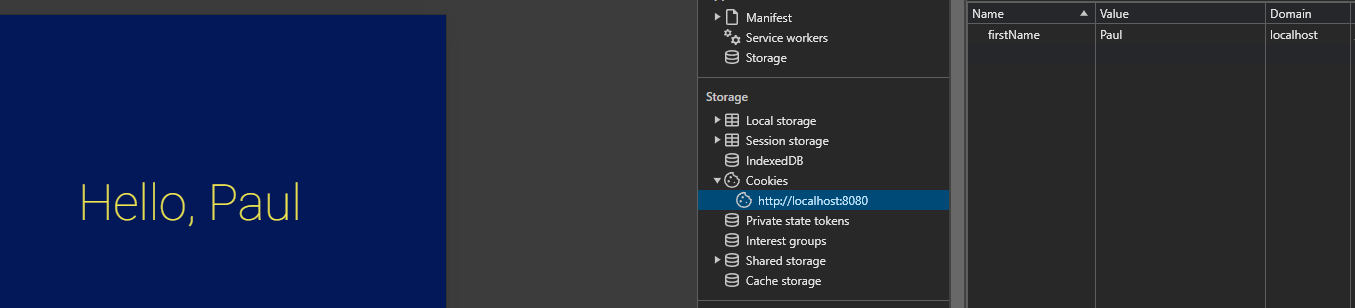
\includegraphics[width=0.7\textwidth]{image/sbCookie}
    \caption{Cookie stocké sur l'ordinateur de l'utilisateur}
    \label{fig:sbCookie}
\end{figure}

Elle a dû être hébergée sur un serveur Web, ce qui a permis de découvrir la conteneurisation (mettre l'application dans un conteneur), l’orchestration (gérer plusieurs conteneurs) ainsi que le déploiement continu (mettre à jour l'application automatiquement).

Pour empêcher que l'application soit victime de cyber-attaques, nous avons appliqué de bonnes pratiques de sécurité, comme cacher les clés API et les URLs sensibles en utilisant des variables d'environnement ou des secrets.

\section{Conception}

\subsection{Formation et apprentissage}

Dans un premier temps, afin de réaliser ce projet, l’essentiel était de se former sur JavaScript.
De plus, étant donné qu’à l’IUT nous faisions du JavaScript, cela m’a permis de progresser plus rapidement.
En parallèle, j’ai dû comprendre et apprendre le fonctionnement du Framework Angular et comment créer une API CRUD (une interface qui permet de créer, lire, mettre à jour et supprimer des données dans une base de données).

\subsection{Développement}

Une fois les connaissances acquises, j’ai pu commencer à développer l’application. L’application est divisée en deux parties :

\begin{itemize}
    \item \textbf{FrontEnd} : La partie visible de l’application, réalisée avec Angular.
    \begin{figure}[H]
        \centering
        \begin{minipage}{.6\textwidth}
            \centering
            \begin{lstlisting}[language=Java]
getFirstName(): Observable<{ string }> {
    const firstName = this.cookieService.get('firstName');
    return this.http.get<{ firstName: string }>(
      `${this.apiUrl}/firstName?cookie=${firstName}`
    );
}
            \end{lstlisting}
            \caption{Exemple de code du FrontEnd : Récupération du prénom via un service de cookies et une requête HTTP GET.}
        \end{minipage}
    \end{figure}

    \item \textbf{BackEnd} : La partie qui fonctionne côté serveur, réalisée avec Node.js.
    \begin{figure}[H]
        \centering
        \begin{minipage}{.6\textwidth}
            \centering
            \begin{lstlisting}[language=Java]
app.get('/backend/firstName', async (req, res) => {
  const userId = req.query.userId;
  console.log("ID de l'utilisateur dans la requête :", userId);
  if (!userId) {
    res.json({
    'World'
});
    return;
  }
  try {
    const user = await User.findById(userId);
    console.log('Utilisateur récupéré depuis MongoDB :', user);
    if (!user) {
      res.json({ firstName: 'World' });
      return;
    }
    res.json({ firstName: user.firstName });
  } catch (error) {
    console.error('Erreur lors de la récupération du prénom depuis MongoDB :', error);
    res.status(500).json({ error: 'Erreur lors de la récupération du prénom.' });
  }
});
            \end{lstlisting}
            \caption{Exemple de code du BackEnd : Récupération du prénom de l'utilisateur depuis la base de données.}
        \end{minipage}
    \end{figure}
\end{itemize}

Le développement a pris du temps, avec des erreurs et des retours en arrière fréquents, mais cela m'a beaucoup motivé et m'a donné envie de progresser.
Une fois le développement terminé, nous avons acquis de nombreuses compétences et nous étions prêts pour le déploiement.

\section{Déploiement}

Le déploiement consiste à mettre l’application en ligne sur un serveur.
Le chercheur m’a fourni un serveur cloud sécurisé par une connexion SSH. Il m’a donné des instructions afin de me former, et m'a recommandé de conteneuriser l’application sous forme de conteneur Docker.

\begin{figure}[H]
    \centering
    \begin{minipage}{.8\textwidth}
        \centering
        \begin{lstlisting}[language=Go]
 FROM node:18.18.0
 WORKDIR /app
 COPY package*.json ./
 RUN npm install -g npm@10.2.1
 RUN npm install
 RUN npm audit fix
 EXPOSE 3000
 COPY app.js .
 COPY config.json .
 CMD ["node", "app.js"]
        \end{lstlisting}
        \caption{Exemple de code d'un fichier Docker pour conteneuriser le backend.}
    \end{minipage}
\end{figure}

Les conteneurs sont légers et faciles à transporter, ce qui optimise l’espace et permet de faire fonctionner l’application directement sur le serveur. Le chercheur s’est occupé de la partie infrastructure, en mettant en place un DNS pour vérifier si l’application fonctionnait. Après avoir réalisé la première partie du déploiement et appliqué les bonnes pratiques de cybersécurité, nous avons pu ajouter des fonctionnalités supplémentaires pour augmenter la difficulté et améliorer l’application.

\section{Amélioration de l’application}

Le chercheur m'a fait découvrir Kubernetes, une technologie très utilisée pour le déploiement et l'orchestration de conteneurs. Kubernetes permet d'orchestrer des conteneurs, gérer leur cycle de vie, et assurer le bon fonctionnement de l'application grâce à des outils de déploiement continu. En utilisant Kubernetes, j'ai pu mettre en place un déploiement continu de manière simple et efficace pour automatiser au mieux les tâches répétitives.

\section{Conclusion}

Une fois le déploiement finalisé et fonctionnel, le chercheur a jugé que nous pouvions partir sur un projet plus concret et complet. Ce projet était très pédagogique mais peu concret d’un point de vue professionnel. Il m’a permis de découvrir comment réaliser un projet et quelles sont les étapes pour y arriver. De plus, il m’a poussé à me renseigner sur toutes les technologies que j’ai été amené à utiliser. Ce projet a été un très bon point de départ car il n’a pas été complexe dans sa forme mais il permet de pratiquer de nombreux domaines de compétences dans le DevOps. J’ai apprécié réaliser ce projet, et malgré les difficultés rencontrées, je reste passionné.

    \pagestyle{fancy} % Appliquer l'en-tête personnalisé à partir de ce point

    \chapter{Projet Find Your Teams}

\section{Introduction}

Le second projet est aussi guidé par le chercheur, mais avec une approche complètement différente.
C’est une approche « Startups » où nous avons cherché un domaine que nous apprécions et nous avons essayé de résoudre un problème existant dans ce domaine.
Pour ce projet, nous avons choisi un domaine que nous aimons : le sport.
Nous n'avions jamais entendu parler d'un réseau social permettant de trouver un partenaire ou un club pour s'entraîner dans n'importe quel sport.
Après quelques recherches, nous avons constaté qu'il n'existait pas encore une telle application sur le marché.
Ce projet a pour principal objectif de renforcer et d'augmenter les compétences déjà acquises sur le projet Bac à Sable.

\section{Technologies utilisées}

\begin{multicols}{2}
    \begin{itemize}
        \item Angular : Un framework JavaScript qui facilite la création d'applications Web interactives.
        \item Node.js : Un environnement d'exécution JavaScript côté serveur.
        \item TypeScript : Un langage de programmation qui est une extension de JavaScript.
        \item Go : Un langage de programmation simple et performant.
        \item MongoDB : Une base de données utilisée dans les applications Web.
        \item GitHub Actions : Un service pour automatiser diverses tâches telle que le déploiement.
        \item GitHub : Une plateforme de développement collaborative basée sur Git.
        \item Google Cloud Platform : Une suite de services cloud proposée par Google.
        \item Terraform : Un outil d'infrastructure en tant que code (IaC).
        \item Google Cloud Run : Un service qui permet d'exécuter des conteneurs Docker.
        \item Google Cloud Build : Un service qui permet d'automatiser la construction d’applications.
        \item Google Cloud Artifact Registry : Un service qui permet de stocker des images de conteneurs.
        \item Google Cloud Secret Manager : Un service de gestion des secrets.
        \item Google Cloud DNS : Un service pour gérer et résoudre les noms de domaine.
    \end{itemize}
\end{multicols}

\section{Objectif du projet}

L’approche startup signifie qu’avant de commencer la partie de développement, il faut analyser ce qui existe, ce qui a fonctionné et ce qui fonctionne à l’heure actuelle. Il faut également analyser le marché, définir les objectifs de l’application, son design, sa maquette et ensuite développer. L’objectif de l’application est de permettre à un utilisateur de créer un événement sportif, d'afficher une carte des événements et d'avoir un canal de message.

\section{Conception}

\subsection{Première conception de l’application}

Pour la première partie du développement, le chercheur m’a laissé développer à ma manière afin de voir ma gestion de projet individuel.
J’ai voulu réaliser tous les éléments souhaités dans l’application et y rajouter des idées que j’avais sur le moment.
Très vite, j’avais plein d’idées mais pas encore très concrètes, et j’étais un peu perdu. Le chercheur m’a donc expliqué qu’il fallait avoir une approche minimaliste pour déployer au plus vite, en se concentrant sur les fonctionnalités minimales de l’application. Nous avons utilisé une méthode de « refactoring » pour rendre le code réutilisable et minimaliste.

\subsection{Développement des fonctionnalités nécessaires}

Je me suis concentré sur le développement des fonctionnalités nécessaires au fonctionnement de l’application :
\begin{itemize}
    \item Une carte interactive listant chaque événement.
    \begin{figure}[H]
        \centering
        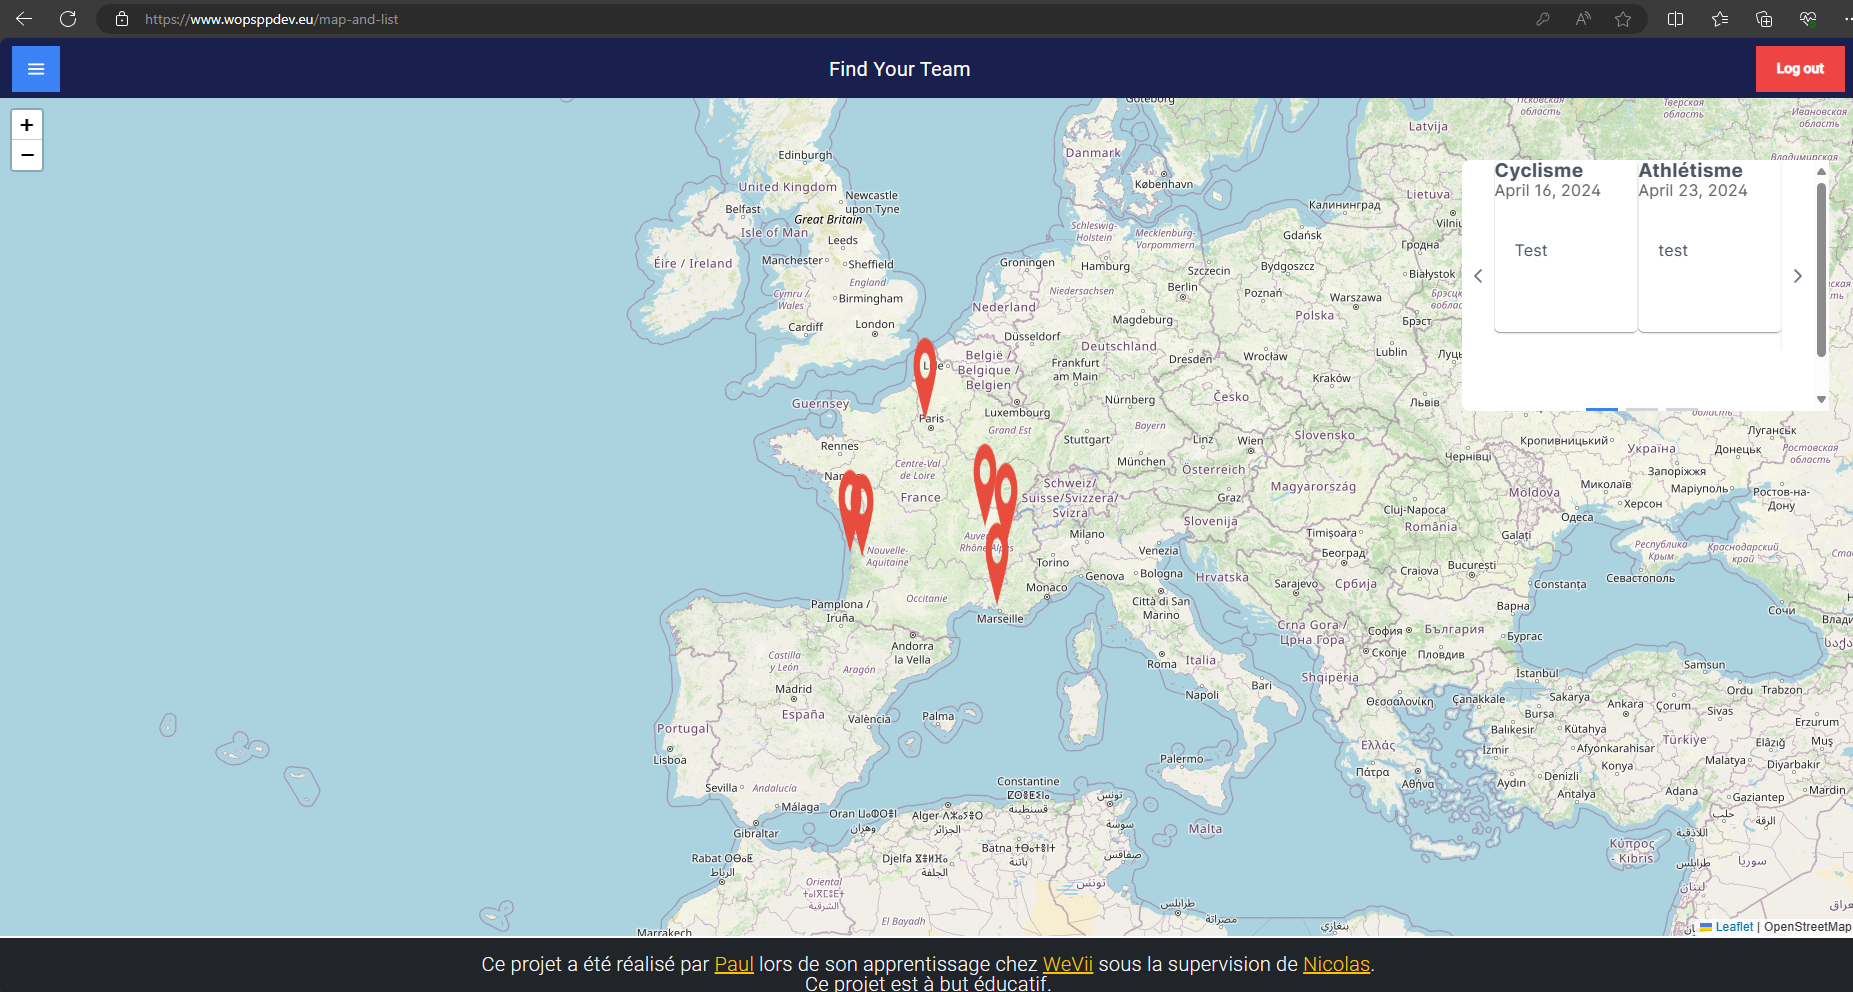
\includegraphics[width=0.45\textwidth]{image/fytMap}
        \caption{Carte interactive des évènements}
        \label{fig:fytMap}
    \end{figure}
    \item Un formulaire permettant d’ajouter un événement.
    \begin{figure}[H]
        \centering
        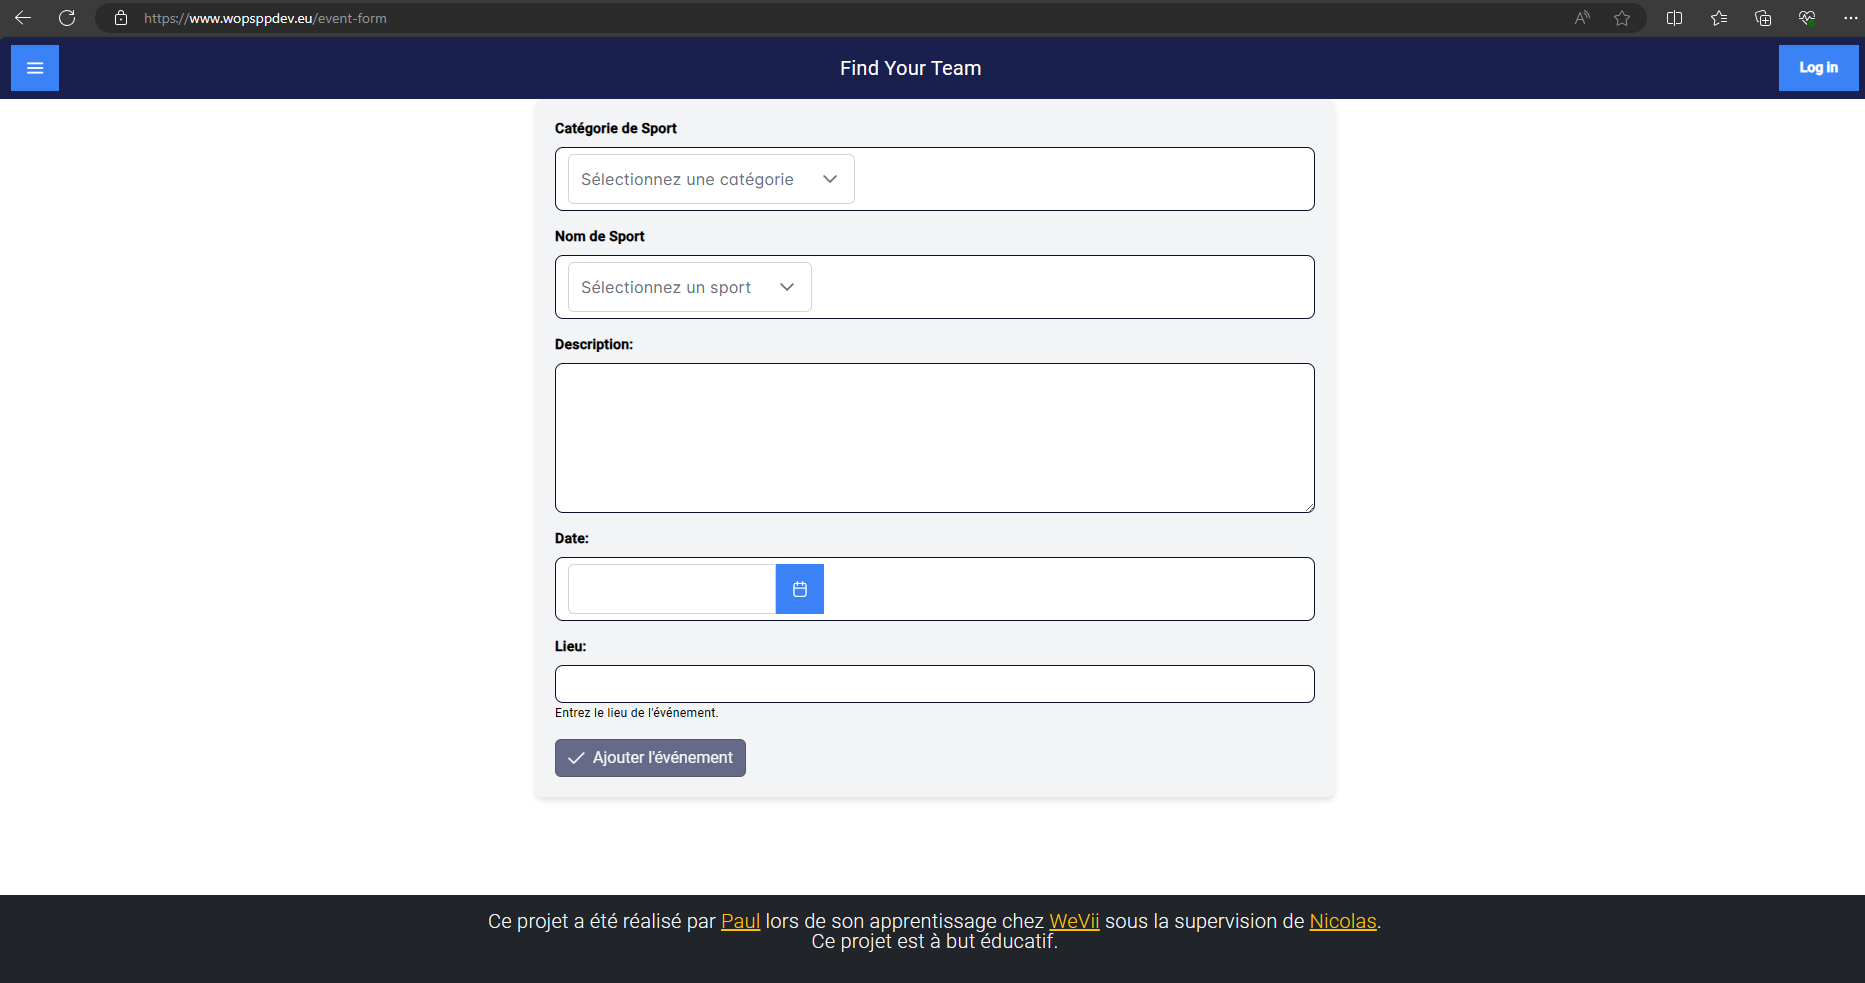
\includegraphics[width=0.45\textwidth]{image/fytForm}
        \caption{Formulaire d'ajout d'événement}
        \label{fig:fytForm}
    \end{figure}
    \item Une liste des évènements permettant au créateur de l’événement de modifier ou supprimer l’événement.
\end{itemize}

Une fois l’application développée de manière minimaliste, j'ai créé une instance de machine virtuelle (VM), un nom de domaine et conteneurisé mon application.
Commencer à déployer sur une VM permet de faire du diagnostic réseau et d’avoir la main sur tout en cas de problème.
Une fois le déploiement réussi, il faut mettre en place un déploiement continu pour automatiser ce processus, car le déploiement est une tâche répétitive.
Pour cela, j’ai choisi GitHub Actions qui permet de faire un déploiement directement avec SSH et d'y mettre ses instructions.

\section{Amélioration de l’application}

J'ai recueilli les retours des utilisateurs extérieurs au projet pour connaître leurs avis sur l’application.
Voici un exemple de retour reçu :
\begin{figure}[H]
    \centering
    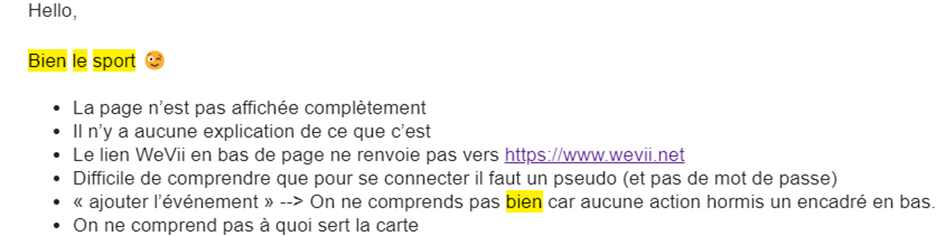
\includegraphics[width=\textwidth]{image/bienLeSportFYT}
    \caption{Commentaire sur l'application}
    \label{fig:commentaire_application}
\end{figure}

Les utilisateurs avaient du mal à comprendre l'application, j'ai donc ajouté une page d'accueil pour mieux expliquer son fonctionnement.
\begin{figure}[ht]
    \centering
    \begin{minipage}{.45\textwidth}
        \centering
        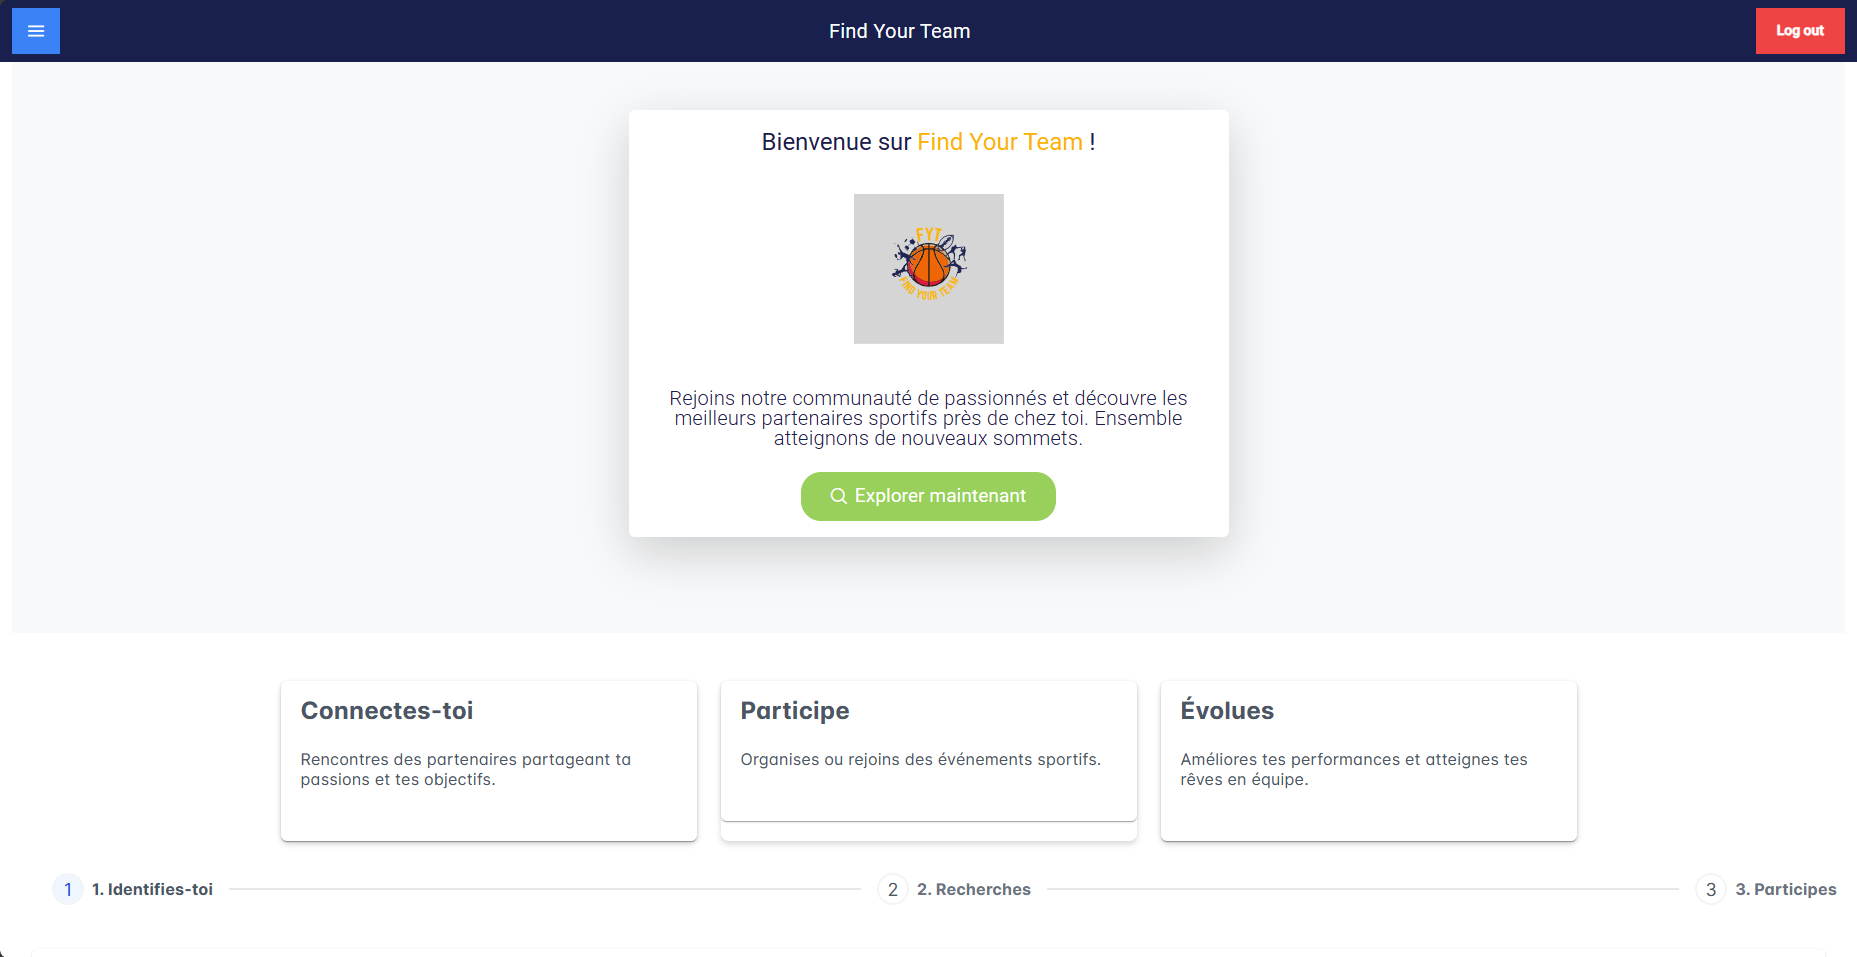
\includegraphics[width=\linewidth]{image/fytLandingPage}
        \caption{Page d'accueil lors de la connexion}
        \label{fig:fytlp}
    \end{minipage}%
    \hfill
    \begin{minipage}{.45\textwidth}
        \centering
        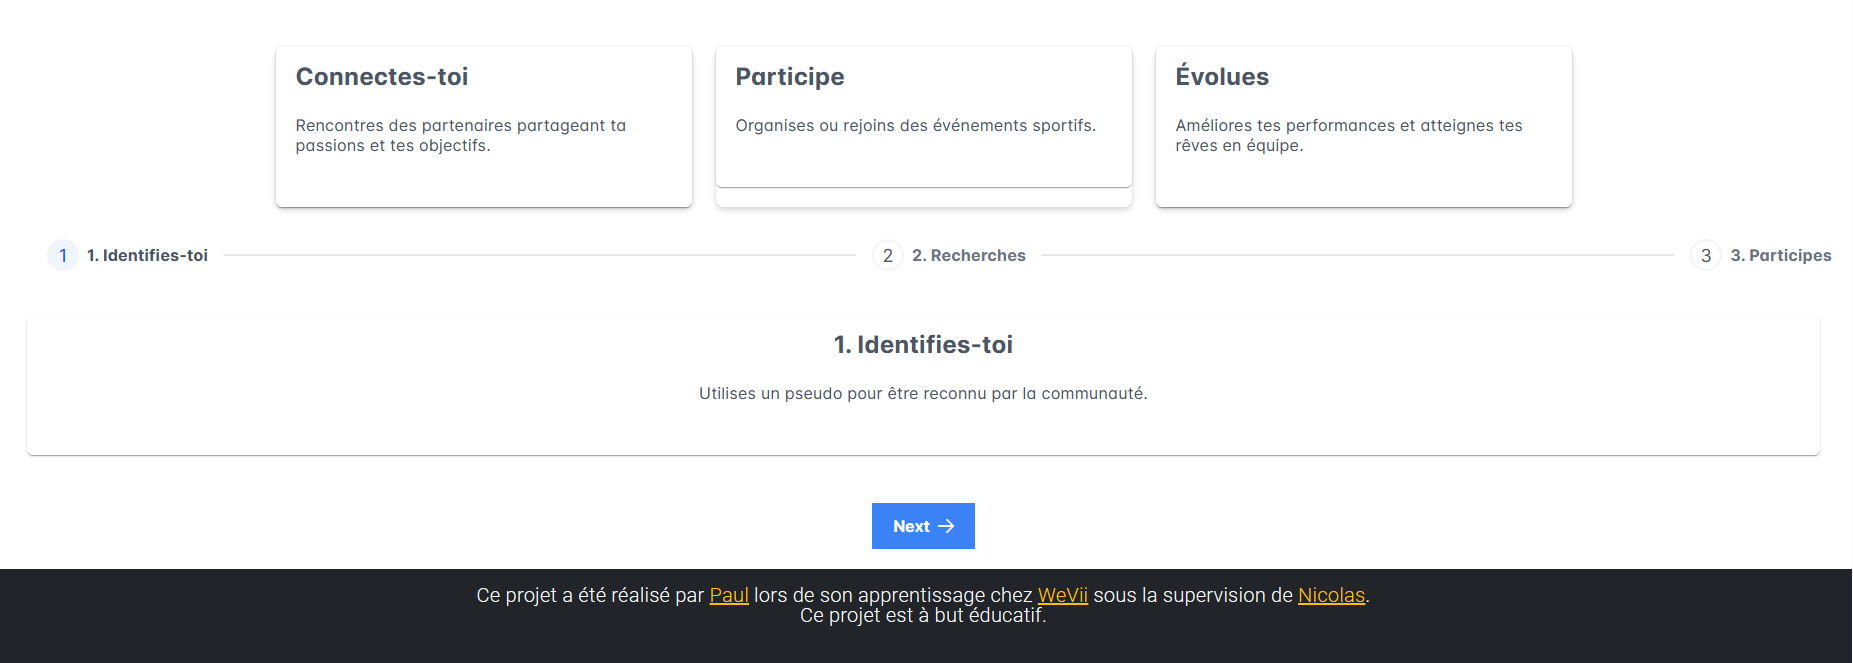
\includegraphics[width=\linewidth]{image/fytLandingPageFooter}
        \caption{Partie basse de la page d'accueil}
        \label{fig:fytlpfooter}
    \end{minipage}
\end{figure}

Les utilisateurs voulaient également un système d'authentification. Plutôt que de créer le système moi-même, j'ai utilisé Auth0, un service d'authentification facile à intégrer.
\begin{figure}[H]
    \centering
    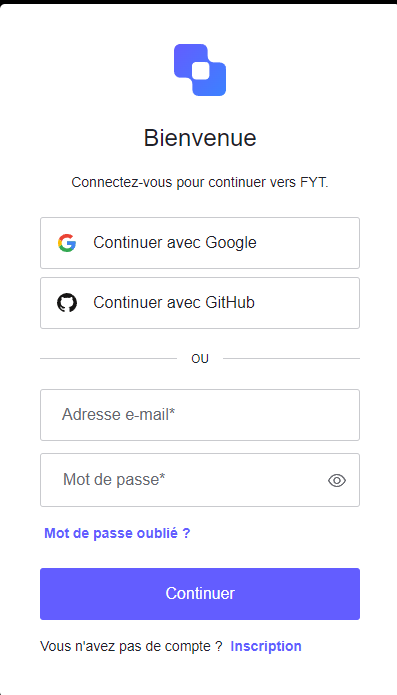
\includegraphics[width=0.35\textwidth]{image/fytAuth}
    \caption{Authentification avec Auth0}
    \label{fig:fytAuth}
\end{figure}

J'ai dû corriger des erreurs d'interface utilisateur, notamment la synchronisation entre l'ajout d'un élément et son affichage sur la carte.
Nous avions des cours sur la qualité du développement, où nous avons appris comment rendre le code plus facile à maintenir, avec des principes comme SOLID et les design patterns.
Cela m'a poussé à refactoriser le code pour le rendre plus clair et fonctionnel, par exemple en séparant le formulaire et l'affichage des événements en deux routes différentes.

\section{Déploiement et Automatisation}

Pour le déploiement, j'ai utilisé Google Cloud Run, qui exécute directement un conteneur.
J'ai également utilisé Google Cloud Artifact Registry pour stocker les images de conteneur, Cloud Build pour construire l'image automatiquement lors du déploiement continu, et Cloud Deploy pour tout déployer avec un fichier YAML.
\begin{figure}[H]
    \centering
    \begin{minipage}{.8\textwidth}
        \centering
        \begin{lstlisting}[language=Go, basicstyle=\ttfamily\scriptsize]
steps:
  - name: 'gcr.io/cloud-builders/git'
    args: ['ls', '-la', '.'] # test

  # install node package
  - name: 'node'
    entrypoint: 'npm'
    args: [ 'install' ]

  # Build Node App
  - name: 'node'
    entrypoint: 'npm'
    args: [ 'run', 'build' ]

  # Docker Build
  - name: 'gcr.io/cloud-builders/docker'
    args:
      [
        'build',
        '-t',
        ImageDocker,
        '-f',
        'Dockerfile',
        '.',
      ]

  # Docker Push to Google Artifact Registry
  - name: 'gcr.io/cloud-builders/docker'
    args: ['push', ImageDocker]

  - name: 'hashicorp/terraform'
    args: ['init']
    env: ['GOOGLE_CREDENTIALS=/workspace/account.json']

  - name: 'hashicorp/terraform'
    args: ['apply', '-auto-approve']
    env: ['GOOGLE_CREDENTIALS=/workspace/account.json']

availableSecrets:
  secretManager:
    - versionName: LienVersion
      env: 'GOOGLE_CREDENTIALS'

    # Deploy to Cloud Run
- name: 'gcr.io/cloud-builders/gcloud'
  args:
    [
      'run',
      'deploy',
      'cloudrunservice',
      '--image',
      ImageDocker,
      '--region',
      'us-central1',
      '--platform',
      'managed',
    ]
        \end{lstlisting}
        \caption{Exemple de code du fichier cloudbuild.yaml}
    \end{minipage}
\end{figure}

Google Cloud Run fourni une URL pour le service. J'ai utilisé Cloud DNS pour rediriger vers mon service Google Run pour le frontend. Mon frontend et mon backend communiquent via une API CRUD. Pour automatiser cela, j'ai créé un service en Go qui récupère l'URL du backend.
\begin{figure}[H]
    \centering
    \begin{minipage}{.8\textwidth}
        \centering
        \begin{lstlisting}[language=Go, basicstyle=\ttfamily\scriptsize]
import (
    "context"
    "github.com/gin-contrib/cors"
    "github.com/gin-gonic/gin"
    "microservice.com/appfyt/gcp"
    "net/http"
)

func getURLByName(c *gin.Context) {
    name := c.Param("name")
    c.IndentedJSON(http.StatusOK, gcp.GetURLByName(gcp.ListServicesRequest(gcp.ConnectToGCP(context.Background()), context.Background()), name))
}

func getAllUrlAndName(c *gin.Context) {
    c.IndentedJSON(http.StatusOK, gcp.GetAllUrl(gcp.ListServicesRequest(gcp.ConnectToGCP(context.Background()), context.Background())))
}

func LauncServ() {
    r := gin.Default()
    r.Use(cors.New(cors.Config{
        AllowOrigins:     []string{"*"},
        AllowMethods:     []string{"GET", "POST", "PUT", "DELETE", "OPTIONS"},
        AllowHeaders:     []string{"Origin"},
        ExposeHeaders:    []string{"Content-Length"},
        AllowCredentials: true,
    }))

    r.GET("/service/:name", getURLByName)
    r.GET("/service", getAllUrlAndName)
    r.Run(":3000")
}
        \end{lstlisting}
        \caption{Exemple de code du Service Go pour récupérer l'URL du backend}
    \end{minipage}
\end{figure}

Pour déployer ce service, j'ai utilisé Terraform, qui permet de coder l'architecture souhaitée et de créer automatiquement l'infrastructure nécessaire.
\begin{figure}[H]
    \centering
    \begin{minipage}{.8\textwidth}
        \centering
        \begin{lstlisting}[language=Go, basicstyle=\ttfamily\scriptsize]
resource "google_cloud_run_service" "microserviceurl" {
  name     = var.serviceName
  location = var.region

  template {
    spec {
      containers {
        image = var.imageMicroserviceurl
      }
    }
  }

  autogenerate_revision_name = true
}
        \end{lstlisting}
        \caption{Exemple de code Terraform pour déployer le service Go}
    \end{minipage}
\end{figure}

\section{Conclusion}

Ce projet m’a fait découvrir de nombreuses facettes du monde de l’informatique telles que le développement, le déploiement, la gestion d’une infrastructure, la sécurité ainsi que l’automatisation.
Tout ceci m’a permis de comprendre et de me rendre compte des domaines et compétences que j’apprécie et que je souhaite améliorer.

J’aime le développement avec une préférence pour le développement BackEnd.
J’ai adoré utiliser le langage Go et je souhaite m’expertiser dans ce langage.
Le développement FrontEnd n’est pas ma partie favorite car elle demande des compétences en design que je n’ai pas et qui ne me plaisent pas particulièrement.

La sécurité est une partie obligatoire et essentielle pour chaque domaine, donc il est important de connaître les bonnes pratiques en termes de cybersécurité afin de réaliser des applications et des architectures sécurisées.
La gestion de l'infrastructure, le déploiement et l'automatisation peuvent être réalisés avec du code.
C'est une partie très intéressante, surtout combinée avec le développement backend.
Cela permet d'augmenter la productivité et d'être autonome dans la mise en production des applications.

Ce projet m'a donc confirmé que je souhaite travailler dans le domaine du DevOps, qui combine développement et opérations pour améliorer et automatiser les processus de déploiement.

\clearpage

    \pagestyle{fancy} % Appliquer l'en-tête personnalisé à partir de ce point

    \chapter*{Conclusion}
\addcontentsline{toc}{chapter}{Conclusion}
\begin{center}
    Cette première expérience professionnelle m’a été bénéfique sur différents points.

    \bigskip

    Tout d’abord, d’un point de vue technique, car j’ai appris de nombreuses choses dans le domaine de l’informatique, mais aussi d’un point de vue personnel, car j’ai découvert la conscience professionnelle, la rigueur et l’importance de la régularité.
    Mes compétences et connaissances ont grandement augmenté durant l’année entre septembre 2023 et maintenant.

    \bigskip

    Le principe de l’alternance consiste à alterner entre étudier à l’iut Paris Rives de Seine et travailler chez WeVii.
    Selon moi ce principe s’est avéré très enrichissante des deux cotés.
    D’un côté l’iut apporte un enseignant transversal tel que le droit, l’anglais, le management… Mais aussi une approche très théorique de ce que l’on peut pratiquer en entreprise ceci permet de comprendre plus en profondeur la partie technique mais aussi de comprendre le fonctionnement de l’entreprise grâce aux matières transversales.
    De l’autre côté l’entreprise permet d’avancer davantage sur les points techniques et apporte une pratique régulière qui favorise l’apprentissage.

    \bigskip

    Pour ma part, l’alternance m’a permis d’évoluer en termes de compétences mais aussi en connaissances et ainsi de constater plus facilement mon évolution personnelle.

    \bigskip

    Le fait de constater sa propre évolution personnelle entre chaque projet permet de s’intéresser d’autant plus à ces derniers.
    Dans l’informatique les projets sont nombreux et peuvent être très variés.
    Ce que j’aime dans ce domaine, c’est la pratique constante qui permet d’évoluer chaque jour.
    Grâce à cela, nous pouvons constater une réelle évolution tout en continuant d’apprendre quotidiennement, peu importe le projet ou le domaine.

    \bigskip

    À la suite de cette année, je souhaite poursuivre en école d'ingénieur, toujours en tant qu'alternant chez WeVii, tout en me spécialisant dans le domaine du DevOps avec un focus sur le Cloud.
    Cependant, certains aspects me restent à découvrir, comme le travail dans une grande équipe composée de développeurs, de designers, de testeurs et de managers.
    J'aimerais appliquer d'autres méthodes de travail et en particulier les méthodes agiles.
    Je souhaite réaliser des projets avec des contraintes plus importantes que celles de cette année, car je pense que cela serait une expérience enrichissante et m'apporterait de nouvelles compétences.

    \bigskip

    Plus tard, dans ma vie professionnelle, je souhaite continuer dans l'architecture cloud et le DevOps.
    Cette année a renforcé mes choix.
    Je voudrais faire un peu de salariat, mais aussi être indépendant, pour avoir du temps pour enseigner dans des domaines techniques, sous forme de conférences ou de cours.
    Je pense que l'enseignement pourrait me plaire, mais je ne me vois pas y consacrer toute ma vie.
    Cependant, enseigner entre 10 et 15 heures par semaine pourrait être une expérience très enrichissante.

\end{center}
\clearpage
    \pagestyle{fancy} % Appliquer l'en-tête personnalisé à partir de ce point

    \chapter*{Glossaire Technique}
\addcontentsline{toc}{chapter}{Glossaire Technique}
\begin{multicols}{2}
    \section*{A}

    \subsection*{Angular}
    \begin{itemize}
        \item Un framework JavaScript qui utilise TypeScript pour le développement d'applications Frontend.
    \end{itemize}

    \subsection*{API CRUD}
    \begin{itemize}
        \item Un ensemble de services permettant de créer, lire, mettre à jour et supprimer des données (CRUD signifie Create, Read, Update, Delete).
    \end{itemize}

    \subsection*{ArgoCD}
    \begin{itemize}
        \item Un outil de déploiement continu pour Kubernetes.
    \end{itemize}

    \section*{B}

    \subsection*{Backend}
    \begin{itemize}
        \item La partie serveur du développement, non visible pour un utilisateur.
    \end{itemize}

    \section*{D}

    \subsection*{DevOps}
    \begin{itemize}
        \item Une méthodologie combinant le développement logiciel (Dev) et les opérations informatiques (Ops) pour améliorer la collaboration et l'efficacité.
    \end{itemize}

    \subsection*{Docker}
    \begin{itemize}
        \item Un logiciel qui utilise la technologie de conteneurisation pour permettre aux applications de fonctionner de manière cohérente sur différents environnements.
    \end{itemize}

    \subsection*{DNS}
    \begin{itemize}
        \item Système de noms de domaine, un service qui convertit les noms de domaine lisibles par les humains en adresses IP lisibles par les machines.
    \end{itemize}

    \section*{F}

    \subsection*{FrontEnd}
    \begin{itemize}
        \item Les éléments visibles par l'utilisateur dans une application ou un site web.
    \end{itemize}

    \subsection*{Framework}
    \begin{itemize}
        \item Une boîte à outils pour les développeurs qui fournit des fonctionnalités prêtes à l'emploi et des règles à suivre pour gagner du temps.
    \end{itemize}

    \section*{G}

    \subsection*{Git}
    \begin{itemize}
        \item Un système de contrôle de version qui permet de suivre les modifications apportées au code source.
    \end{itemize}

    \subsection*{GitHub}
    \begin{itemize}
        \item Un site web qui permet de stocker du code en utilisant la technologie Git.
    \end{itemize}

    \subsection*{GitHub Actions}
    \begin{itemize}
        \item Un service d'automatisation et de déploiement continu intégré à GitHub.
    \end{itemize}

    \subsection*{Go (Golang)}
    \begin{itemize}
        \item Un langage de programmation créé par Google, compilé et fortement typé, avec une syntaxe simple d'utilisation.
    \end{itemize}

    \subsection*{Google Cloud Artifact Registry}
    \begin{itemize}
        \item Un service de Google Cloud Platform pour stocker des images de conteneurs.
    \end{itemize}

    \subsection*{Google Cloud Build}
    \begin{itemize}
        \item Un service de Google Cloud Platform pour automatiser la construction d'applications.
    \end{itemize}

    \subsection*{Google Cloud DNS}
    \begin{itemize}
        \item Un service de Google Cloud Platform pour gérer et résoudre les noms de domaine.
    \end{itemize}

    \subsection*{Google Cloud Platform}
    \begin{itemize}
        \item Une suite de services cloud proposés par Google.
    \end{itemize}

    \subsection*{Google Cloud Run}
    \begin{itemize}
        \item Un service de Google Cloud Platform pour exécuter des conteneurs Docker.
    \end{itemize}

    \subsection*{Google Cloud Secret Manager}
    \begin{itemize}
        \item Un service de gestion des secrets de Google Cloud Platform pour stocker et gérer de manière sécurisée des informations sensibles.
    \end{itemize}

    \section*{H}

    \subsection*{Helm}
    \begin{itemize}
        \item Un outil de gestion des applications Kubernetes qui facilite le déploiement et la gestion des applications sur Kubernetes.
    \end{itemize}

    \section*{J}

    \subsection*{JavaScript}
    \begin{itemize}
        \item Un langage de programmation principalement utilisé pour créer des scripts sur les pages web afin de les rendre interactives.
    \end{itemize}

    \section*{K}

    \subsection*{Kubernetes}
    \begin{itemize}
        \item Un outil qui automatise le déploiement, la gestion et la mise à l'échelle des conteneurs d'applications.
    \end{itemize}

    \section*{M}

    \subsection*{MongoDB}
    \begin{itemize}
        \item Une base de données NoSQL utilisée pour stocker des informations.
    \end{itemize}

    \section*{N}

    \subsection*{Node.js}
    \begin{itemize}
        \item Un environnement qui permet d'exécuter du code JavaScript côté serveur.
    \end{itemize}

    \section*{S}

    \subsection*{Serveur Cloud}
    \begin{itemize}
        \item Un ordinateur virtuel qui exécute des applications sur Internet.
    \end{itemize}

    \subsection*{SSH (Secure Shell)}
    \begin{itemize}
        \item Un protocole de communication sécurisé utilisant un chiffrement asymétrique pour se connecter de manière sécurisée à un serveur.
    \end{itemize}

    \section*{T}

    \subsection*{Terraform}
    \begin{itemize}
        \item Un outil d'infrastructure en tant que code (IaC) qui permet de définir et de gérer des infrastructures cloud avec des fichiers de configuration.
    \end{itemize}

    \subsection*{TypeScript}
    \begin{itemize}
        \item Une surcouche de JavaScript qui ajoute des types statiques pour rendre le code plus sécurisé et maintenable.
    \end{itemize}

    \section*{U}

    \subsection*{URL}
    \begin{itemize}
        \item Uniform Resource Locator, une adresse web qui spécifie l'emplacement d'une ressource sur Internet.
    \end{itemize}

    \section*{Y}

    \subsection*{YAML}
    \begin{itemize}
        \item Un langage de sérialisation de données facile à lire et à écrire utilisé pour les fichiers de configuration.
    \end{itemize}
\end{multicols}

\clearpage
    \chapter*{Bibliographie et Webographie}
\addcontentsline{toc}{chapter}{Bibliographie et Webographie}

\begin{itemize}
    \item \textbf{Mozilla Developer Network (MDN)} \\
    \url{https://developer.mozilla.org/} \\
    Ressource pour HTML, CSS, JavaScript, TypeScript, Angular, Node.js, HTTP\@.

    \item \textbf{Red Hat} \\
    \url{https://www.redhat.com/} \\
    Documentation sur Kubernetes, Docker, DevOps, Terraform, Cloud.

    \item \textbf{ResearchGate} \\
    \url{https://www.researchgate.net/publication/357163866_Observability_and_resources_managements_in_cloud-native_environnements} \\
    Ressource pour l'observabilité et la gestion des ressources dans les environnements cloud-native.

    \item \textbf{Roadmap.sh} \\
    \url{https://roadmap.sh/} \\
    Outil pour situer ses compétences.

    \item \textbf{Google Cloud Documentation} \\
    \url{https://cloud.google.com/docs?hl=fr} \\
    Documentation sur Google Cloud Run.

    \item \textbf{Overleaf} \\
    \url{https://fr.overleaf.com/latex/templates} \\
    Outil de rédaction collaborative pour LaTeX afin de trouver des idées de modèles pour le rapport\@.
\end{itemize}


\end{document}
